%% This Beamer template is based on the one found here: https://github.com/sanhacheong/stanford-beamer-presentation, and edited to be used for Stanford ARM Lab

\documentclass[10pt]{beamer}
%\mode<presentation>{}

\usepackage{media9}
\usepackage{amssymb,amsmath,amsthm,enumerate}
\usepackage{mathtools}
\usepackage[utf8]{inputenc}
\usepackage{array}
\usepackage[parfill]{parskip}
\usepackage[utf8]{vietnam}
\usepackage{graphicx,animate}
\usepackage{caption}
\usepackage{subcaption}
\usepackage{bm}
\usepackage{amsfonts,amscd}
\usepackage[]{units}
\usepackage{listings}
\usepackage{multicol}
\usepackage{multirow}
\usepackage{tcolorbox}
\usepackage{physics}
\usepackage{movie15}
% Enable colored hyperlinks
\hypersetup{colorlinks=true}

\usefonttheme{professionalfonts}

% The following three lines are for crossmarks & checkmarks
\usepackage{pifont}% http://ctan.org/pkg/pifont
\newcommand{\cmark}{\ding{51}}%
\newcommand{\xmark}{\ding{55}}%

% Numbered captions of tables, pictures, etc.
\setbeamertemplate{caption}[numbered]
\usepackage{media9} 
%\usepackage[superscript,biblabel]{cite}
%\usepackage{algorithmic}
%\usepackage{algorithm2e}
%\usepackage{algpseudocode}
\usepackage[linesnumbered,ruled,vlined]{algorithm2e}
%\usepackage{algorithm}
%\usepackage{algorithmic}
%\usepackage{caption}
\usepackage[font=scriptsize,justification=centering]{caption}
%\usepackage{xcolor}
\usepackage{array}
%\renewcommand{\thealgocf}{}

\usepackage[natbib,backend=biber,style=ieee, sorting=ynt]{biblatex}
\bibliography{ref.bib}

\usepackage[acronym]{glossaries}

\usepackage{graphicx}
\graphicspath{{./figures}}
\usepackage{hyperref}

\usepackage{pythonhighlight}

\setbeamertemplate{theorems}[numbered]
\theoremstyle{remark}
\newtheorem{dl}{Định lý}
\newtheorem{md}{Mệnh đề}
\newtheorem{bd}{Bổ đề}
\newtheorem{dn}{Định nghĩa}
\newtheorem{hq}{Hệ quả}
%\theoremstyle{definition}

\numberwithin{algocf}{section}
\numberwithin{equation}{section}
\numberwithin{dl}{section}
\numberwithin{figure}{section}


%\newcommand{\empy}[1]{{\color{darkorange}\emph{#1}}}
%\newcommand{\empr}[1]{{\color{cardinalred}\emph{#1}}}
%\newcommand{\examplebox}[2]{
%\begin{tcolorbox}[colframe=darkcardinal,colback=boxgray,title=#1]
%#2
%\end{tcolorbox}}

%\usetheme{Stanford} 
%\input{./style_files_stanford/my_beamer_defs.sty}
\usetheme{Copenhagen}
\usecolortheme{seahorse}
%\logo{
\includegraphics[height=0.5in]{logos/HUS-name.jpg}}

\makeatletter
\let\@@magyar@captionfix\relax
\makeatother

\title[Kiến trúc lập trình song song và phân tán]{Kiến trúc lập trình song song và phân tán với OpenMP - MPI - CUDA}

\AtBeginSection[]
{
    \begin{frame}
        \frametitle{Nội dung}
        \tableofcontents[currentsection, subsectionstyle=show/show/hide]
    \end{frame}
}

\setbeamertemplate{page number in head/foot}[totalframenumber]
\setbeamertemplate{frametitle continuation}{}

\begin{document}
\author[Nguyễn Chí Thanh - 21007925]{
	\begin{tabular}{c} 
	\Large
	Nguyễn Chí Thanh \\
    \footnotesize \href{mailto:nguyenchithanh\_sdh21@hus.edu.vn}{nguyenchithanh\_sdh21@hus.edu.vn}
\end{tabular}
\vspace{-4ex}}

\institute{
	\vskip 5pt
	\begin{figure}
		\centering
		\begin{subfigure}[t]{0.5\textwidth}
			\centering
			
\includegraphics[height=0.75in]{logos/HUS-logo.jpg}
		\end{subfigure}%
		~ 
		\begin{subfigure}[t]{0.5\textwidth}
			\centering
			
\includegraphics[height=0.75in]{logos/MIM-logo.png}
		\end{subfigure}
	\end{figure}
	\vskip 5pt	
	Đại học Quốc Gia Hà Nội \\
	Trường đại học Khoa học tự nhiên\\
	Khoa Toán - Cơ - Tin học
	\vskip 3pt
}

%\begin{noheadline}
\begin{frame} \maketitle \end{frame}
%\end{noheadline}
    
\setbeamertemplate{itemize items}[default]
\setbeamertemplate{itemize subitem}[circle]

\begin{frame}{Nội dung}
    \tableofcontents[hidesubsections]
\end{frame}

\section{OpenMP}

\begin{frame}{Giới thiệu OpenMP}
    \begin{itemize}
        \item OpenMP là một API viết các ứng dụng đa luồng bộ nhớ chia sẻ sử dụng ngôn ngữ C/C++ hoặc Fortran
        \item Gồm có các chỉ thị biên dịch, runtime routine, biến môi trường.
        \item Hội đồng phát triển và phê duyệt kiến trúc OpenMP:
        \begin{itemize}
            \item Duy trì spec OpenMP
            \item Thành viên chính: AMD, Cray, Fujitsu, HP, IBM, Intel, Oracle, NVIDIA, Microsoft, Tesxas Instruments, Convey
            \item Thành viên ngắn hạn: ANL,	ASC/LLNL, cOMPunity, EPCC, LANL, NASA, TACC, RWTH, Aachen University, UH
        \end{itemize}
    \end{itemize}
\end{frame}

\begin{frame}{Các thành phần của OpenMP}
    \begin{columns}[onlytextwidth]
        \begin{column}{0.3\textwidth}
            Các chỉ thị biên dịch:
            \begin{itemize}
                \item Parallel region	
                \item Worksharing constructs
                \item Tasking
                \item Offloading
                \item Affinity
                \item Error Handling
                \item SIMD
                \item Synchronization
                \item Data-sharing attributes
            \end{itemize}
        \end{column}
        \begin{column}{0.3\textwidth}
            Các biến runtime:
            \begin{itemize}
                \item Số luồng
                \item Thread ID 
                \item Dynamic thread adjustment
                \item Nested parallelism
                \item Schedule
                \item Active levels
                \item Thread limit
                \item Nesting level
                \item Ancestor thread
                \item Team size 
                \item Locking
                \item Wallclock timer
            \end{itemize}
        \end{column}
        \begin{column}{0.3\textwidth}
            Các biến môi Trường:
            \begin{itemize}
                \item Số luồng
                \item Scheduling type
                \item Dynamic thread adjustment
                \item Nested parallelism
                \item Stacksize
                \item Idle threads
                \item Active levels
                \item Thread limit
            \end{itemize}
        \end{column}
    \end{columns}
\end{frame}

\begin{frame}
    \begin{figure}[H]
        \centering
        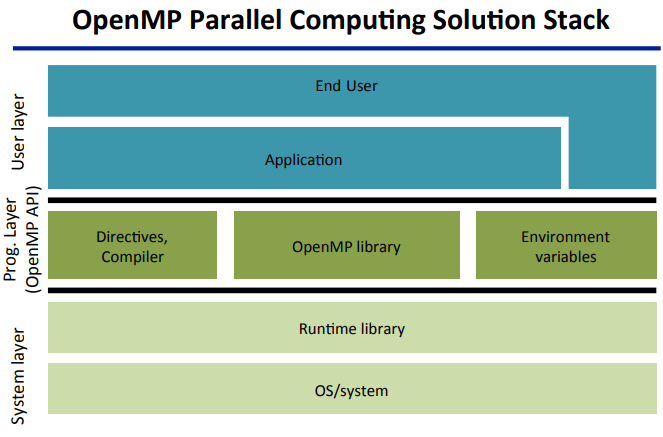
\includegraphics[width=0.9\linewidth]{figures/OpenMP/OpenMP_Parallel_Computing_Solution_Stack.png}
        \caption{Vị trí OpenMP trong stack}
    \end{figure}
\end{frame}

\begin{frame}{Chỉ thị biên dịch}
    \begin{itemize}
        \item Chỉ thị thực thi OpenMP áp dụng cho các khối có cấu trúc đứng kế tiếp với nó.
        \item Một chỉ thị bắt đầu với \#pragma omp. Các phần còn lại tuân theo quy ước của ngôn ngữ C và C++ cho các chị thị biên dịch 
    \end{itemize}
\end{frame}

\begin{frame}{Một số chỉ thị biên dịch của OpenMP}
    \begin{itemize}
        \item \#pragma omp parallel
        \item \#pragma omp for
        \item \#pragma omp sections
        \item \#pragma omp parallel shared/private
        \item \#pragma omp barrier
    \end{itemize}
\end{frame}

\begin{frame}{Mô hình thực thi Fork-Join của OpenMP}
    \begin{figure}[H]
        \centering
        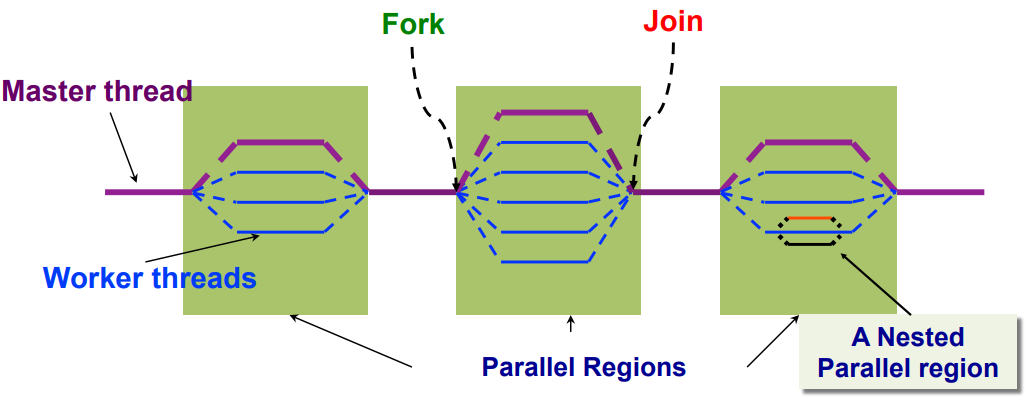
\includegraphics[width=\linewidth]{figures/OpenMP/Fork_Join_Execution_Model.png}
        \caption{Mô hình thực thi Fork-Join của OpenMP}
    \end{figure}
\end{frame}

\begin{frame}{Mô hình bộ nhớ của OpenMP}
    \begin{columns}[onlytextwidth]
        \begin{column}{0.5\linewidth}
            \begin{figure}[H]
                \centering
                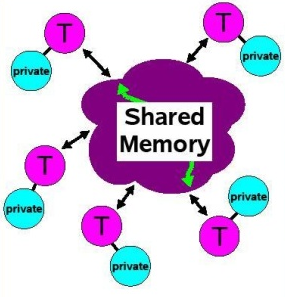
\includegraphics[width=\linewidth]{figures/OpenMP/OpenMP_Shared_Memory_Model.png}
            \end{figure}
        \end{column}
        \begin{column}{0.5\linewidth}
            \begin{itemize}
                \item Tất cả các luồng có cùng bộ nhớ chia sẻ toàn cục.
                \item Dữ liệu có thể chia sẻ hoặc riêng tư giữa các luồng
                \item Dữ liệu chia sẻ có thể truy cập từ tất cả các luồng
                \item Dữ liệu riêng tư chỉ có thể được truy cập từ luồng sở hữu dữ liệu
                \item Chia sẻ dữ liệu trong suốt với lập trình viên
                \item Có đồng bộ hóa, chủ yếu ngầm diễn ra.
            \end{itemize}
        \end{column}
    \end{columns}
    
\end{frame}

\begin{frame}[fragile]{OpenMP parallel region}
    Trong C/C++: một khối là một biểu thức hoặc một nhóm biểu thức giữa cặp ngoặc { }.
    \begin{columns}[onlytextwidth]
        \begin{column}{0.5\linewidth}
            \begin{verbatim}
#pragma omp parallel
{
    id = omp_get_thread_num();
    res[id] = lots_of_work(id);
}
            \end{verbatim}
        \end{column}
        \begin{column}{0.5\linewidth}
            \begin{verbatim}
#pragma omp parallel for
for(i=0;i<N;i++) {
    res[i] = big_calc(i);
    A[i] = B[i] + res[i];
} 
            \end{verbatim}
        \end{column}
    \end{columns}
\end{frame}

\begin{frame}{Chạy thực thi}
    \begin{itemize}
        \item Đặt biến môi trường OMP\_NUM\_THREADS.
        \item Chạy lệnh: g++ -fopenmp -g ./input.c -o ./input
    \end{itemize}
\end{frame}

\begin{frame}[fragile]{Chương trình đơn giản OpenMP}
    \begin{verbatim}
        #include <stdio.h>
        #include <omp.h>

        int main(int argc, char** argv) {
            #pragma omp parallel
            {
                printf("Hello World\n");
            } // End of parallel region 
            return 0;
        }
    \end{verbatim}
    Thực thi chương trình:
    \begin{verbatim}
        g++ -fopenmp -g ./hello_openmp.c -o ./hello_openmp
        ./hello_openmp
    \end{verbatim}
\end{frame}

\begin{frame}[fragile]{Khối lệnh có cấu trúc}
    \begin{itemize}
        \item Khối lệnh có cấu trúc: Một điểm vào và một điểm ra.
        \item Trong C/C++: một khối lệnh là một câu lệnh đơn hoặc một nhóm các câu lệnh giữa các ngoặc.
    \end{itemize}

    \begin{columns}[onlytextwidth]
        \begin{column}{0.5\textwidth}
            \begin{verbatim}
#pragma omp parallel
{
id = omp_get_thread_num(); 
A[id] = big_compute(id);
}		
            \end{verbatim}
        \end{column}
        \begin{column}{0.5\textwidth}
            \begin{verbatim}
#pragma omp for
for (int i=0;i<N;i++) {
    res[i] = big_calc(i);
    A[i] = B[i] + res[i]; 
}
            \end{verbatim}
        \end{column}
    \end{columns}
\end{frame}

\begin{frame}[fragile]{Cách viết rút gọn chỉ thị}
    Hai cách viết sau là tương đương:
    \begin{columns}[onlytextwidth]
        \begin{column}{0.5\textwidth}
            \begin{verbatim}
int i;
double res[MAX];
#pragma omp parallel				
{
    #pragma omp for
    for (i=0;i< MAX; i++) {
        res[i] = huge();
    } 
}
            \end{verbatim}
        \end{column}
        \begin{column}{0.5\textwidth}
            \begin{verbatim}
int i;
double res[MAX];
#pragma omp parallel for					
for (i=0;i< MAX; i++) {
    res[i] = huge();
}
            \end{verbatim}
        \end{column}
    \end{columns}
\end{frame}

\begin{frame}[fragile]{Đặt số luồng thực thi}
    Cách 1:
    \begin{verbatim}
export OMP_NUM_THREADS=4
    \end{verbatim}
    Cách 2:
    \begin{verbatim}
omp_set_num_threads(4);
    \end{verbatim}
\end{frame}

\begin{frame}[fragile]{Minh họa quá trình chạy song song}
    \begin{columns}[onlytextwidth]
        \begin{column}{0.5\textwidth}
            \begin{verbatim}
...A... 
#pragma omp parallel
{
    foo(); /* ...B... */
}
...C... 
#pragma omp parallel
{
...D...
}
...E...
            \end{verbatim}
        \end{column}
        \begin{column}{0.5\textwidth}
            \begin{figure}[H]
                \centering
                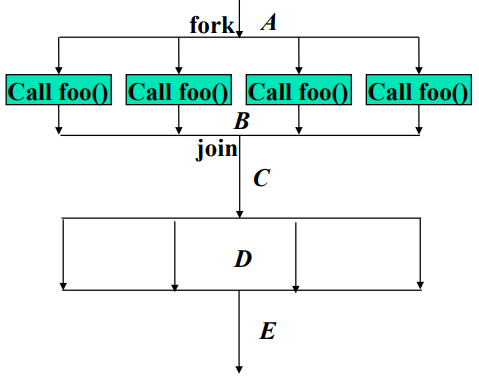
\includegraphics[width=\linewidth]{figures/OpenMP/Fork.png}
            \end{figure}
        \end{column}
    \end{columns}
\end{frame}

\begin{frame}[fragile]{Nguyên lý thiết kế}
    \begin{verbatim}
#pragma omp parallel
{
    int thread_id = omp_get_thread_num();
    int num_threads = omp_get_num_threads();
    printf("Thread %d of %d\n", thread_id, num_threads); 
}
    \end{verbatim}
    \begin{itemize}
        \item Từng hàm printf() là một tác vụ
        \item Parallel region tập hợp một tập các luồng cho tính toán và xử lý.
        \item Từng luồng thực thi một tác vụ đơn lẻ
        \item Ánh xạ 1:1 giữa các tác vụ và luồng
    \end{itemize}
\end{frame}

\begin{frame}[fragile]{Cú pháp OpenMP}
    \begin{itemize}
        \item OpenMP sử dụng các chỉ thị biên dịch dạng \#pragma.
        \item Với C và C++, chỉ thị có dạng:
        \begin{verbatim}
#pragma omp construct [clause [clause]...]
        \end{verbatim}
        \item Khai báo tệp tiêu đề: \#include <omp.h>
    \end{itemize}
\end{frame}

\begin{frame}[fragile]{Mô hình chương trình SIMD}
    \begin{itemize}
        \item SIMD cho parallel region:
        \begin{itemize}
            \item Tất cả các luồng của parallel region cùng thực thi một đoạn code.
            \item Mỗi luồng có một ID riêng
        \end{itemize}
        \item Có thể sử dụng threadID để phân nhánh thực thi các luồng, các luồng khác nhau có thể theo những con đường khác nhau qua cùng đoạn code:
        \begin{verbatim}
if(thread_id == x) {

} else {

}
        \end{verbatim}
        \item SIMD được sử dụng rất phổ biến cho cấu trúc các chương trình song song: OpenMP, MPI, CUDA,...
    \end{itemize}
\end{frame}

\begin{frame}[fragile]{Phân nhánh parallel regions}
    Chỉ có luồng master in ra màn hình số luồng
        \begin{verbatim}
#pragma omp parallel
 {
    int thread_id = omp_get_thread_num(); 
    int num_threads = omp_get_num_threads();
    if (thread_id == 0) 
        printf("Thread %d of %d\n", thread_id, num_threads); 
    else 
        printf("Thread %d\n", thread_id);
 }
        \end{verbatim}
\end{frame}

\begin{frame}[fragile]{Phân nhánh parallel regions}
    Chỉ có luồng master đọc số luồng và tất cả các luồng cùng in ra số luồng
    \begin{verbatim}
#pragma omp parallel
{
    int thread_id = omp_get_thread_num();
    if (thread_id == 0)
        num_threads = omp_get_num_threads();
    #pragma omp barrier
    printf("Thread %d of %d\n", thread_id, num_threads); 
}
    \end{verbatim}
\end{frame}

\begin{frame}{Chỉ thị Barrier}
    \begin{figure}[H]
        \centering
        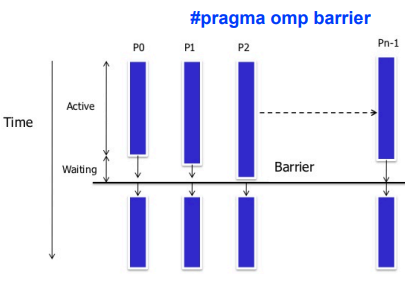
\includegraphics[width=0.9\linewidth]{figures/OpenMP/Barrier.png}
        \caption{Đồng bộ hóa giữa các luồng}
    \end{figure}
\end{frame}

\begin{frame}[fragile]{Chỉ thị Barrier}
    \begin{verbatim}
#pragma omp parallel shared (A, B, C) private(id)
{
    id=omp_get_thread_num();
    A[id] = big_calc1(id);
    #pragma omp barrier
    #pragma omp for
    for(i = 0;i < N; i++){
        C[i] = big_calc3(I, A);
    }
    // Có một barrier ngầm định kết thúc vòng lặp for
    #pragma omp for nowait // loại bỏ barrier
    for(i=0; i < N; i++){ 
        B[i] = big_calc2(C, i); 
    }
    A[id] = big_calc3(id);
} // Một barrier ngầm định kết thúc parallel region
    \end{verbatim}
\end{frame}

\begin{frame}[fragile]{Chỉ thị master}
    \begin{itemize}
        \item Ký hiệu khối lệnh chỉ được thực thi bởi luồng master
        \item Các luồng khác bỏ qua
        \item Không có đồng bộ hóa ngầm định
    \end{itemize}
    \begin{verbatim}
#pragma omp parallel private (tmp)
{
    do_many_things_together();
    #pragma omp master
    { 
        exchange_boundaries_by_master_only (); 
    }
    #pragma barrier
    do_many_other_things_together();
} 
    \end{verbatim}
\end{frame}

\begin{frame}[fragile]{Chỉ thị single}
    \begin{itemize}
        \item Ký hiệu khối lệnh chỉ được thực thi bởi một luồng
        \item Một barrier được ngầm định ở cuối khối lệnh
    \end{itemize}
    \begin{verbatim}
#pragma omp parallel private (tmp)
{
    do_many_things_together();
    #pragma omp single
    { 
        exchange_boundaries_by_one(); 
        }
    do_many_other_things_together();
}
    \end{verbatim}
\end{frame}

\begin{frame}[fragile]{Phân chia công việc sử dụng thread id}
    \begin{figure}[H]
        \centering
        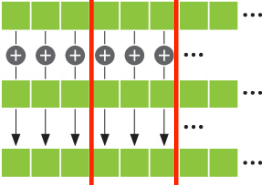
\includegraphics[width=0.3\linewidth]{figures/OpenMP/Distribute.png}
    \end{figure}
    \begin{verbatim}
        #pragma omp parallel shared (a, b)
        {
            int id, i, Nthrds, istart, iend;
            id = omp_get_thread_num();
            Nthrds = omp_get_num_threads();
            istart = id * N / Nthrds;
            iend = (id+1) * N / Nthrds;
            for(i=istart;i<iend;i++) { 
                a[i] = a[i] + b[i]; 
            }
        } 
    \end{verbatim}
\end{frame}

\begin{frame}[fragile]{Các mệnh đề schedule}
    Mệnh đề schdule được dùng để xác định cách chia vùng dữ liệu trong các vòng lặp giữa các luồng
    \begin{itemize}
        \item schedule (static | dynamic | guided [,chunk\_size])
        \item schedule (auto | runtime)
    \end{itemize}
    \begin{itemize}
        \item static chia các lặp lại của một vòng lặp thành các phần có kích thước bằng nhau và gán một phần cho mỗi luồng.
        Kích thước các phần được xác định tại thời điểm biên dịch và duy trì không đổi trong suốt quá trình thực thi của vòng lặp.
        \item dynamic gán các đoạn nhỏ của dữ liệu cho các luồng tại thời điểm chạy.
        Mỗi luồng thực hiện phần được gán và yêu cầu đoạn tiếp theo khi hoàn thành (các đoạn nhỏ kích thước bằng nhau).
        Kích thước các đoạn dữ liệu do từng luồng đảm nhận khác nhau.
        \item guided tương tự như dynamic nhưng các đoạn dữ liệu nhỏ do từng luồng đảm nhận giảm theo hàm mũ.
    \end{itemize}
\end{frame}

\begin{frame}[fragile]{Các mệnh đề schedule}

    \begin{itemize}
        \item auto cho phép OpenMP tự động chọn lịch trình phù hợp dựa trên điều kiện của runtime.
        Lịch trình được đưa ra bởi hệ thống.
        \item runtime cho phép lịch trình và chunk\_size xác định tại thời điểm chạy sử dụng biến môi trường.
    \end{itemize}
    \begin{verbatim}
#pragma omp parallel for schedule(static) private(id)
for(i = 0; i < N; i++) {
    A[i] = B[i] + C[i];
}
    \end{verbatim}
\end{frame}

\begin{frame}{Các mệnh đề schedule}
    \begin{figure}[[H]]
        \centering
        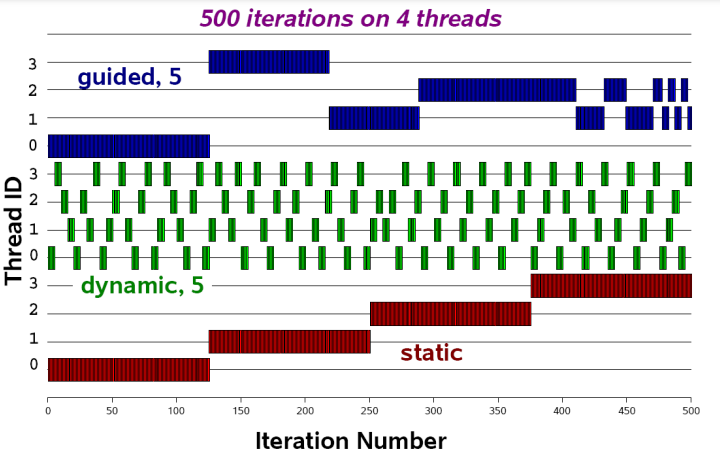
\includegraphics[width=0.8\linewidth]{figures/OpenMP/Schedule_Modes_Comparison.png}
        \caption{So sánh các chế độ schedule}
    \end{figure}
\end{frame}

\begin{frame}[fragile]{Chỉ thị sections}
    Mỗi section được gán cho một thread
    \begin{verbatim}
#pragma omp parallel
#pragma omp sections
{
    #pragma omp section
    printf("1 + 1, id: %d\n", omp_get_thread_num());
    #pragma omp section
    printf("1 + 2, id: %d\n", omp_get_thread_num());
    #pragma omp section
    printf("1 + 3, id: %d\n", omp_get_thread_num());
}
    \end{verbatim}

    Một barrier ngầm định ở cuối khối omp sections.
    Có thể tắt barrier sử dụng từ khóa nowait.
\end{frame}

\begin{frame}[fragile]{Chỉ thị sections}
    \begin{verbatim}
#pragma omp parallel private(id)
{
    int id = omp_get_thread_num();
    #pragma omp sections nowait
    {
        #pragma omp section
        printf("1 + 1, id: %d\n", id);
        #pragma omp section
        printf("1 + 2, id: %d\n", id);
        #pragma omp section
        printf("1 + 3, id: %d\n", id);
    }
    printf("%d\n", id);
}
    \end{verbatim}
\end{frame}

\begin{frame}[fragile]{Loop Collapse}
    \begin{itemize}
        \item Cho phép song song hóa giữa các vòng lặp lồng nhau mà không cần dùng song song hóa lồng nhau.
        \item Mệnh đề collapse chỉ thị bao nhiêu vòng lặp bị collapse
    \end{itemize}
    \begin{verbatim}
#pragma omp parallel for collapse(2)
for (i = 0; i < M; i++) {
    for (j = 0; j < P; j++) {
        int temp = 0;
        for (k = 0; k < N; k++) {
            temp += *(B + i * N + k) * *(C + k * P + j);
        }
        *(A + i * P + j) = temp;
    }
}
    \end{verbatim}
\end{frame}

\subsection{Môi trường dữ liệu}

\begin{frame}{Môi trường dữ liệu}
    \begin{itemize}
        \item Hầu hết các biến được chia sẻ giữa các luồng
        \item Các biến toàn cục, static mặc định là chia sẻ
        \item Các biến cục bộ trong hàm được gọi trong parallel region hoặc các biến được khai báo trong parallel region là riêng tư.
        \item shared, private, firstprivate, lastprivate?
    \end{itemize}
\end{frame}

\begin{frame}{Mệnh đề private}
    \begin{itemize}
        \item Mệnh đề private khai báo một biến là riêng tư đối với mỗi luồng trong một parallel region.
        \item Các biến riêng có các phiên bản riêng cho từng luồng và mỗi luồng hoạt động với bản sao riêng của biến đó.
        \item Giá trị ban đầu của một biến riêng tư không được xác định, vì vậy nó cần được khởi tạo rõ ràng ở trong luồng.
        \item Sau khi kết thúc parallel region, giá trị biến ban đầu được trở lại giá trị ban đầu trước khi thực hiện parallel region (chưa được khởi tạo????)
    \end{itemize}
\end{frame}

\begin{frame}{Mệnh đề firstprivate}
    \begin{itemize}
        \item Giống như private nhưng biến riêng tư được khởi tạo bằng giá trị ban đầu của biến ban đầu.
        \item Sau khi kết thúc parallel region, giá trị biến ban đầu được trở lại giá trị ban đầu trước khi thực hiện parallel region (chưa được khởi tạo????)
    \end{itemize}
\end{frame}

\begin{frame}{Mệnh đề lastprivate}
    \begin{itemize}
        \item Giống như firstprivate nhưng giá trị của biến ban đầu sau khi thực hiện parallel region được gán cho giá trị cuối cùng mà một biến riêng tư được gán trong khi thực hiện parallel region.
    \end{itemize}
\end{frame}

\begin{frame}[fragile]{Ví dụ private}
    \begin{verbatim}
int id = 0;
#pragma omp parallel private(id)
{
    id = omp_get_thread_num();
    printf("Thread id %d\n", id);
}
printf("Thread %d id\n", id);
    \end{verbatim}
\end{frame}

\begin{frame}[fragile]{Mệnh đề reduction}
    \begin{itemize}
        \item reduction dùng để thực hiện các phép toán trên một biến được chia sẻ trên nhiều luồng trong một parallel region.
        \item reduction kết hợp các giá trị của biến trên từng luồng và lưu trữ kết quả trên một biến duy nhất
        \item Hay sử dụng khi tính tổng, tích, max, min trên một tập các giá trị.
        \item Hay được sử dụng với vòng lặp for.
        \begin{verbatim}
#pragma omp parallel for reduction(operator: variable)
        \end{verbatim}
    \end{itemize}
\end{frame}

\begin{frame}[fragile]{Mệnh đề reduction}
    \begin{verbatim}
int i = 0;
#pragma omp parallel reduction(*:i)
{
    i=omp_get_num_threads();
    printf("%d\n", i);
} // 1 * 4 * 4 * 4 * 4
printf("result=%d\n", i); 
    \end{verbatim}
\end{frame}

\subsection{Đồng bộ hóa trong OpenMP}
\begin{frame}
    \begin{itemize}
        \item Đồng bộ hóa mức cao:
        \begin{itemize}
            \item critical
            \item atomic 
            \item barrier
            \item ordered
        \end{itemize}
        \item Đồng bộ hóa mức thấp
        \begin{itemize}
            \item flush
            \item locks
        \end{itemize}
    \end{itemize}
\end{frame}

\begin{frame}[fragile]{critical}
    \begin{itemize}
        \item critical chỉ cho phép một luồng duy nhất được thực thi một đoạn code tại một thời điểm
    \end{itemize}

    \begin{verbatim}
int shared = 0;
#pragma omp parallel
{
    int thread_id = omp_get_thread_num();
    #pragma omp for
    for (int i = 0; i < 100; i++) {
        #pragma omp critical
        {
            shared += 1;
            printf("Thread %d: Incrementing shared to %d\n", thread_id, shared);
        }
    }
}
    \end{verbatim}
\end{frame}

\begin{frame}[fragile]{So sánh với single}
    \begin{verbatim}
#pragma omp parallel num_threads(3)
{
   foo();
   bar();
   ...
}
    \end{verbatim}
thread 0: ----< foo() >< bar() >----------->

thread 1: --< foo() >< bar() >------------->

thread 2: ---------< foo() >< bar() >------>
\end{frame}

\begin{frame}[fragile]{So sánh với single}
    \begin{verbatim}
#pragma omp parallel num_threads(3)
{
   #pragma omp single
   foo();
   bar();
   ...
}
    \end{verbatim}
    \begin{verbatim}
thread 0: ------[-------|]< bar() >----->

thread 1: ---[< foo() >-|]< bar() >----->

thread 2: -------------[|]< bar() >----->
    \end{verbatim}
\end{frame}

\begin{frame}[fragile]{So sánh với single}
    \begin{verbatim}
#pragma omp parallel num_threads(3)
{
   #pragma omp single nowait
   foo();
   bar();
   ...
}
    \end{verbatim}
    \begin{verbatim}
thread 0: ------[]< bar() >----------->

thread 1: ---[< foo() >]< bar() >----->

thread 2: -------------[]< bar() >---->
    \end{verbatim}
\end{frame}

\begin{frame}[fragile]{So sánh với single}
    \begin{verbatim}
#pragma omp parallel num_threads(3)
{
   #pragma omp critical
   foo();
   bar();
   ...
}
    \end{verbatim}
    \begin{verbatim}
thread 0: ------xxxxxxxx[< foo() >]< bar() >-------------->

thread 1: ---[< foo() >]< bar() >------------------------->

thread 2: -------------xxxxxxxxxxxx[< foo() >]< bar() >--->
    \end{verbatim}
\end{frame}

\begin{frame}[fragile]{So sánh với single}
    \begin{verbatim}
#pragma omp parallel num_threads(3)
{
   if (omp_get_thread_num() > 1) {
     #pragma omp critical(foo2)
     foo();
   }
   else {
     #pragma omp critical(foo01)
     foo();
   }
   bar();
   ...
}
    \end{verbatim}
    \begin{verbatim}
thread 0: ------xxxxxxxx[< foo() >]< bar() >---->
thread 1: ---[< foo() >]< bar() >--------------->
thread 2: -------------[< foo() >]< bar() >----->
    \end{verbatim}
\end{frame}

\begin{frame}[fragile]{So sánh với single}
    \begin{verbatim}
#pragma omp parallel num_threads(3)
{
   #pragma omp critical
   foo();
   ...
   #pragma omp critical
   bar();
   ...
}
    \end{verbatim}

    \begin{verbatim}
0: ------xxxxxx[<foo()>]< ... >xxxxxxxxxxx[<bar()>]---------->
1: ---[<foo()>]< ... >xxxxxxxxxxx[<bar()>]------------------->
2: -------------xxxxxxxx[<foo()>]< ... >xxxxxxxxxxx[<bar()>]->
    \end{verbatim}
\end{frame}

\begin{frame}[fragile]{atomic}
    \begin{itemize}
        \item atomic là một trường hợp đặc biệt của critical sử dụng cho một số câu lệnh đơn giản
    \end{itemize}

    \begin{verbatim}
int thread_id = omp_get_thread_num();
//#pragma omp for
for (int i = 0; i < 100; i++) {
    #pragma omp critical
    shared += 1;
    printf("Thread %d: Incrementing shared to %d\n", thread_id, shared);
}
    \end{verbatim}
\end{frame}

\begin{frame}[fragile]{ordered}
    \begin{itemize}
        \item ordered bắt buộc vòng lặp thực hiện theo đúng thứ tự trong một parallel region
        \item Đảm bảo các vòng lặp hoặc các đoạn code thực hiện theo đúng thứ tự đưa ra bởi lập trình viên
    \end{itemize}
    \begin{verbatim}
#pragma omp parallel num_threads(4) private(tmp)
#pragma omp for ordered
for (int i = 0; i < 100; i++) {
    tmp = do_in_parallel(i);
    #pragma omp ordered
    printf("i: %d, thread id: %d\n", i, omp_get_thread_num());
}
    \end{verbatim}
\end{frame}

\begin{frame}[fragile]{locks}
    \begin{itemize}
        \item Chỉ cho phép một luồng thực thi một đoạn code tại một thời điểm.
        \item Ngăn khả năng bị race conditions khi nhiều luồng cố gắng truy cập và sửa một dữ liệu được chia sẻ tại cùng một thời điểm.
        \item Sử dụng omp\_lock\_t
        \item Một số hàm hay sử dụng:
        \begin{itemize}
            \item omp\_init\_lock(omp\_lock\_t *): Khởi tạo một khóa
            \item omp\_set\_lock(omp\_lock\_t *): Lấy khóa dành quyền thực thi đoạn code
            \item omp\_unset\_lock(omp\_lock\_t *): Giải phóng khóa cho các luồng khác
            \item omp\_destroy\_lock(omp\_lock\_t *): Hủy khóa
        \end{itemize}
    \end{itemize}
\end{frame}

\begin{frame}[fragile]{locks}
    \begin{verbatim}
omp_lock_t lck;
omp_init_lock(&lck);
int id, tmp;
#pragma omp parallel private (tmp, id)
{
    id = omp_get_thread_num();
    tmp = id * id * id * id;
    omp_set_lock(&lck);
    printf("%d %d\n", id, tmp);
    omp_unset_lock(&lck);
}
omp_destroy_lock(&lck); 
    \end{verbatim}
\end{frame}

\begin{frame}[fragile]{taskwait}
    \begin{itemize}
        \item taskwait giúp cho việc đợi tất cả các tác vụ song song mới thực hiện công việc tiếp theo (bằng một luồng) trong parallel region.
    \end{itemize}

    \begin{verbatim}
#pragma omp parallel num_threads(4)
{
    #pragma omp single
    {
        #pragma omp task
        printf("Task 1 executed by thread %d\n", omp_get_thread_num());
        #pragma omp task
        printf("Task 2 executed by thread %d\n", omp_get_thread_num());
        #pragma omp task
        printf("Task 3 executed by thread %d\n", omp_get_thread_num());
        #pragma omp taskwait
        printf("All tasks completed %d\n", omp_get_thread_num());
    }
}
    \end{verbatim}
\end{frame}

\subsection{Một số hàm thư viện}

\begin{frame}{Một số hàm thư viện}
    \begin{itemize}
        \item void omp\_set\_num\_threads(int);
        \item int omp\_get\_num\_threads(void);
        \item int omp\_get\_thread\_num(void);
        \item int omp\_get\_max\_threads(void);
        \item int omp\_in\_parallel(void);
        \item int omp\_num\_procs(void);	

    \end{itemize}
\end{frame}

\subsection{Một số biến môi trường}
\begin{frame}{Một số biến môi trường}
    \begin{itemize}
        \item Đặt số luồng sử dụng: OMP\_NUM\_THREADS
        \item Điều khiển schedule(runtime): OMP\_SCHEDULE "schedule[, chunk\_size]"
    \end{itemize}
\end{frame}

\subsection{Tối ưu hiệu năng của chương trình viết bằng OpenMP}

\begin{frame}{Hiệu năng của OpenMP}
    \begin{itemize}
        \item OpenMP tương đối dễ sử dụng bằng cách kết hợp các chỉ thị và mệnh đề.
        \item Ta có thể viết một chương trình OpenMP đúng một cách nhanh chóng nhưng là không quan trọng hiệu năng
        \item Khi số luồng lớn chi phí cần để quản lý cũng lớn
    \end{itemize}
\end{frame}

\begin{frame}{Một số vấn đề hiệu năng hay gặp đối với OpenMP}
    \begin{itemize}
        \item Chi phí khởi tạo, quản lý luồng:
        \begin{itemize}
            \item dynamic schedule có chi phí lớn hơn nhiều static
            \item Đồng bộ hóa có chi phí lớn, nếu không thật sự cần thì dùng nowait để tắt barrier
            \item Parallel region lớn giảm overhead, cho phép sử dụng cache và tối ưu hóa
        \end{itemize}
        \item Overhead của các hàm thư viện
        \item Không cân bằng tải giữa các luồng
        \item Không tận dụng tốt cache và chia sẻ dữ liệu bị lỗi
    \end{itemize}
\end{frame}

\begin{frame}{Overheads của một số chỉ thị}
    \begin{figure}[H]
        \centering
        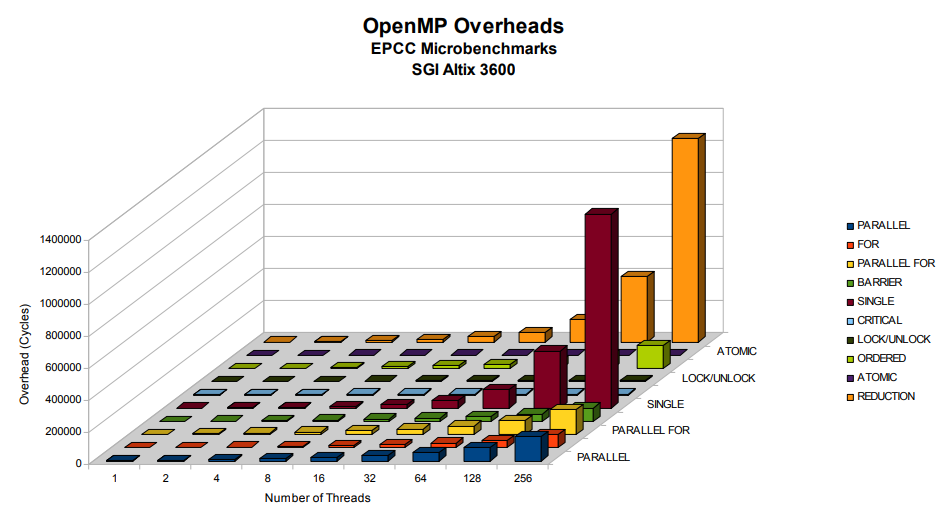
\includegraphics[width=0.8\linewidth]{figures/OpenMP/Overheads_Directives.png}
        \caption{Overheads của một số chỉ thị}
    \end{figure}
\end{frame}

\begin{frame}[fragile]{Một số kỹ thuật tối ưu}
    \begin{itemize}
        \item Giảm tần suất sử dụng barrier với nowait
    \end{itemize}

    \begin{verbatim}
#pragma	omp	parallel	
{	
    #pragma	omp	for
    for(i=0;i<n;i++)	
        ….	
    #pragma	omp	for	nowait
    for(i=0;i<n;i++)	
}	
    \end{verbatim}
\end{frame}

\begin{frame}[fragile]{Một số kỹ thuật tối ưu}
    \begin{verbatim}
#pragma	omp	parallel private(i)	
{	
    #pragma	omp	for	nowait
    for(i=0;i<n;i++)	
        a[i] +=b[i];	
    #pragma	omp	for	nowait
    for(i=0;i<n;i++)	
        c[i] +=d[i];	
    #pragma	omp	barrier	
    #pragma	omp	for	nowait	reducAon(+:sum)	
    for(i=0;i<n;i++)
        sum	+=	a[i]	+	c[i];	
}	
    \end{verbatim}
\end{frame}

\begin{frame}[fragile]{Một số kỹ thuật tối ưu}
    \begin{itemize}
        \item Tránh sử dụng ordered với khối lệnh lớn
        \item Tránh sử dụng critical với khối lệnh lớn
    \end{itemize}
    \begin{verbatim}
    #pragma	omp	parallel shared(a,b) private(c,d)	
    {	
        ...	
        #pragma	omp	critical
        {	
            a += 2*c;	
            c =	d*d; // Nên để biểu thức ra ngoài
        }	
    }	
    \end{verbatim}
\end{frame}

\begin{frame}[fragile]{Một số kỹ thuật tối ưu}
    \begin{itemize}
        \item Parallel regions hãy dài nhất có thể
    \end{itemize}
    \begin{columns}[onlytextwidth]
        \begin{column}{0.5\linewidth}
            \begin{verbatim}
#pragma	omp	parallel		
{	
    #pragma	omp	for	
    for(...) {...}	
}	
opt = opt +	N; // sequential
#pragma	omp	parallel	
{	
    #pragma	omp	for	
    for(...) {...}	
    #pragma	omp	for	
    for(...) {...}	
}    
            \end{verbatim}
        \end{column}
        \begin{column}{0.5\linewidth}
            \begin{verbatim}
#pragma	omp	parallel		
{	
    #pragma	omp	for	
    for(...) {...}	
}
#pragma omp single nowait
opt = opt +	N; // sequential	
#pragma	omp	for	
for(...) {...}	
#pragma	omp	for	
for(...) {...}	
            \end{verbatim}
        \end{column}
    \end{columns}
\end{frame}

\begin{frame}[fragile]{Một số kỹ thuật tối ưu}
    \begin{itemize}
        \item Một parallel region chứa tất cả các vòng lặp for.
    \end{itemize}
    \begin{columns}[onlytextwidth]
        \begin{column}{0.5\linewidth}
            \begin{verbatim}
for (i = 0; i < n; i++)
    for (j = 0; j < n; j++)
        #pragma omp parallel for private(k)
        for (k = 0; k < n; k++) {
            ...
        }
            \end{verbatim}
        \end{column}
        \begin{column}{0.5\linewidth}
            \begin{verbatim}
#pragma omp parallel private(i, j, k)
for (i = 0; i < n; i++)
    for (j = 0; j < n; j++)
        #pragma omp for
        for (k = 0; k < n; k++) {
            ...
        }
            \end{verbatim}
        \end{column}
    \end{columns}
\end{frame}

\begin{frame}[fragile]{Một số kỹ thuật tối ưu}
    \begin{itemize}
        \item Tránh chọn chunk size nhỏ
    \end{itemize}
    \begin{columns}[onlytextwidth]
        \begin{column}{0.5\linewidth}
            \begin{figure}[H]
                \centering
                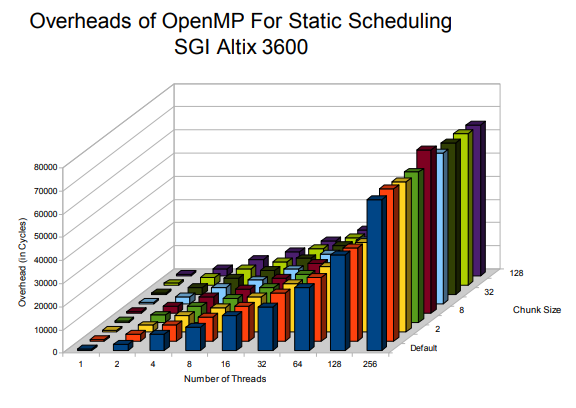
\includegraphics[width=0.9\linewidth]{figures/OpenMP/Overhead_Static_Scheduling_Chunk_Size.png}
            \end{figure}
        \end{column}
        \begin{column}{0.5\linewidth}
            \begin{figure}[H]
                \centering
                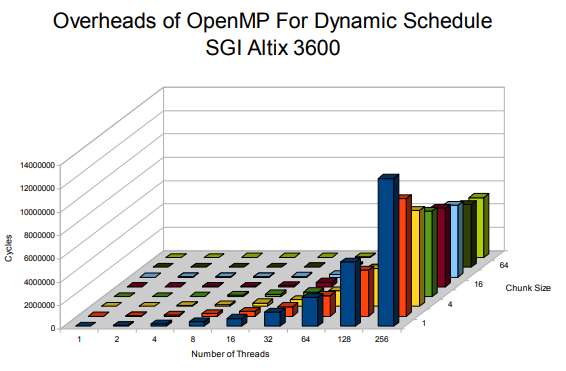
\includegraphics[width=0.9\linewidth]{figures/OpenMP/Overhead_Dynamic_Scheduling_Chunk_Size.png}
            \end{figure}
        \end{column}
    \end{columns}
\end{frame}

\begin{frame}[fragile]{Một số kỹ thuật tối ưu}
    \begin{itemize}
        \item chỉ thị master hiệu quả hơn single nhưng cần thread id 0 sẵn sàng
        \item single hiệu quả hơn nếu thread id 0 không sẵn sàng
        \item single có barrier ngầm, khi không cần thiết nên dùng thêm nowait
    \end{itemize}
\end{frame}

\section{Message Passing Interface}

\subsection{Tổng quan MPI}

\begin{frame}{Tổng quan MPI}
    \begin{itemize}
        \item Là một API tiêu chuẩn cho quá trình truyền thông đẹp, tra cứu thông tin, đăng ký, phân nhóm và tạo mới kiểu dữ liệu thông điệp.
        \item Có thể truyền giao thức theo hai hình thức:
        \begin{itemize}
            \item Truyền điểm - điểm
            \item Truyền quảng bá (một - nhiều, nhiều - một , nhiều - nhiều)
        \end{itemize}
        \item Hỗ trợ lập trình song song mức thấp
        \item Được hỗ trợ trên Fortran 77 và C, MPI2 được hỗ trợ trên C++/Fortran90
        \item Một API rất lớn (128 hàm), MPI-2 có thêm 152 hàm. Đa số người dùng chỉ dùng một phần.
        \item Hướng hiệu năng
    \end{itemize}
\end{frame}

\begin{frame}{Lịch sử MPI}
    \begin{itemize}
        \item Nhiều thư viện truyền thông đẹp đã được tạo ra trong quá khứ:
        \begin{itemize}
            \item TCGMSG, P4, PARMACS, EXPRESS, NX, MPL, PVM
        \end{itemize}
        \item 1992-1994 diễn đàn về truyền thông điệp định nghĩa một tiêu chuẩn mới cho truyền thông điệp (ban đầu đặt là MPPs)
        \item Quá trình phát triển của tiêu chuẩn:
        \begin{itemize}
            \item 1994: MPI 1.0: các giao tiếp cơ bản, Fortran77 và C
            \item 1995: MPI 1.1: sửa lỗi bản trước
            \item 1997: MPI 2.0: Giao tiếp 1 phía, I/O, khởi tạo tiến trình, Fortran 99 và C, giải thích các hàm rõ hơn. Bao gồm MPI 1.2.
            \item 2008: MPI 1.3, 2.1: kết hợp 1.3 và 2.0
            \item 2009: MPI 2.2: sửa lỗi và giải thích các hàm
            \item MPI 3.0 đang trong quá trình chuẩn hóa và hoàn thiện
        \end{itemize}
    \end{itemize}
\end{frame}

\begin{frame}{Bản đồ phát triển}
    \begin{figure}[H]
        \centering
        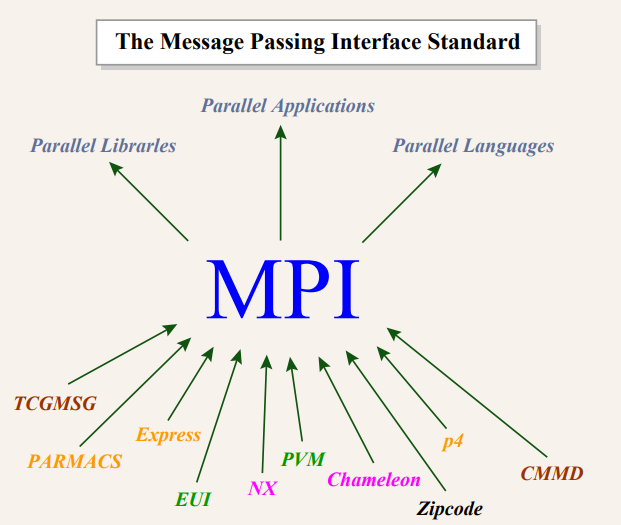
\includegraphics[width=0.75\linewidth]{figures/MPI/MPI_Genealogy.png}
        \caption{Quá trình phát triển của MPI}
    \end{figure}
\end{frame}

\begin{frame}{MPI cơ bản}
    \begin{itemize}
        \item Góc nhìn logic của nền tảng truyền thông điệp:
        \begin{itemize}
            \item p tiến trình
            \item Mỗi tiền trình có một không gian bộ nhớ riêng
        \end{itemize}
        \item Tất cả dữ liệu phải cần được phân chia rõ ràng
        \begin{itemize}
            \item Tiến trình cần truyền dữ liệu
            \item Tiến trình cần nhận dữ liệu
        \end{itemize}
        \item Thường sử dụng mô thức lập trình (SIMD)
        \item Ưu điểm:
        \begin{itemize}
            \item Mô hình hiệu năng đơn giản: chi phí ngầm dễ tính
            \item Hiệu năng và tính linh hoạt cao
        \end{itemize}
        \item Nhược điểm: Mô hình truyền thông điệp hai phía làm chương trình phức tạp
    \end{itemize}
\end{frame}

\begin{frame}{MPI cơ bản}
    \begin{itemize}
        \item File tiêu đề mpi.h cho C/C++ và mpif.h cho Fortran
        \item Tất cả các hàm đều trả về giá trị lỗi
        \item Trong C/C++, các đối số được truyền vào dạng con trỏ
        \item Luôn luôn bắt đầu với MPI\_Init() và kết thúc với MPI\_Finalize() (hoặc MPI\_Abort()).
        Hai hàm trên đều cần được gọi bởi tất cả các tiến trình
        \item Tất cả các hàm, kiểu dữ liệu, hằng số đều có tiền tố là "MPI\_"
        \item Một chương trình MPI có thể chỉ cần sử dụng 6 hàm thư viện
    \end{itemize}
\end{frame}

\begin{frame}{MPI cơ bản}
    \begin{figure}[H]
        \centering
        
\includegraphics[height=0.85\textheight]{figures/MPI/MPI_Full_Routines.png}
    \end{figure}
\end{frame}

\begin{frame}{Một số hàm thông dụng}
    \begin{table}[H]
        \centering
        \begin{tabular}{|l|l|}
            \hline
            MPI\_Init & Khởi tạo môi trường MPI \\
            \hline
            MPI\_Finalize & Ngắt môi trường MPI \\
            \hline
            MPI\_Comm\_size & Xác định số tiến trình \\
            \hline
            MPI\_Comm\_rank & Xác định id của tiến trình gọi hàm trong nhóm \\
            \hline
            MPI\_Send & Truyền thông điệp \\
            \hline
            MPI\_Recv & Nhận thông điệp \\
            \hline
        \end{tabular}
    \end{table}
    
\end{frame}

\begin{frame}{Khởi tạo và ngắt môi trường MPI}
    \begin{itemize}
        \item int MPI\_Init(int *argc, char ***argv) 
        \begin{itemize}
            \item Câu lệnh được gọi trước các hàm khác của MPI
            \item Khởi tạo môi trường MPI
        \end{itemize}
        \item int MPI\_Finalize()
        \begin{itemize}
            \item Được gọi khi kết thúc tính toán
            \item Ngắt môi trường MPI
        \end{itemize}
        \item Mã trả về:
        \begin{itemize}
            \item MPI\_SUCCESS
            \item MPI\_ERROR
        \end{itemize}
    \end{itemize}
\end{frame}

\begin{frame}{Bộ giao tiếp}
    \begin{itemize}
        \item MPI\_Comm: nhóm các tiến trình có thể giao tiếp với nhau
        \item Được truyền vào là đối số của một hàm truyền thông điệp
        \item Một tiến trình có thể thuộc về nhiều nhóm khác nhau
        \item MPI\_COMM\_WORLD: bộ giao tiếp toàn cục bao gồm tất cả các tiến trình
    \end{itemize}
    \begin{figure}[H]
        \centering
        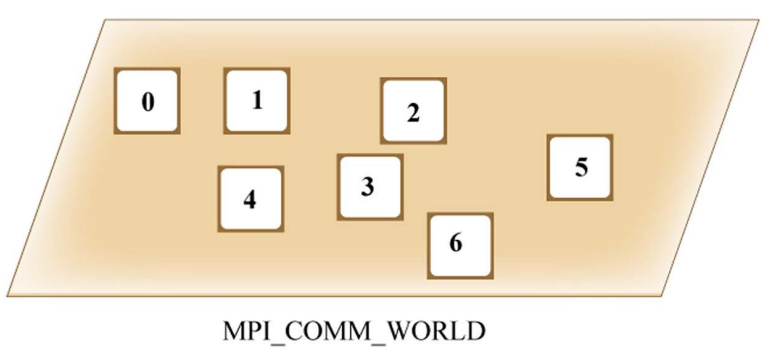
\includegraphics[height=0.4\textheight]{figures/MPI/MPI_COMM_WORLD.png}
    \end{figure}
\end{frame}

\begin{frame}{Truy vấn bộ giao tiếp}
    \begin{itemize}
        \item int MPI\_Comm\_size(MPI\_Comm comm, int *size) : xác định số tiến trình
        \item int MPI\_Comm\_rank(MPI\_Comm comm, int *rank) : xác định chỉ số của tiến tình gọi hàm ($0 \leq rank <$ số tiến trình trong nhóm)
    \end{itemize}
    \begin{figure}[H]
        \centering
        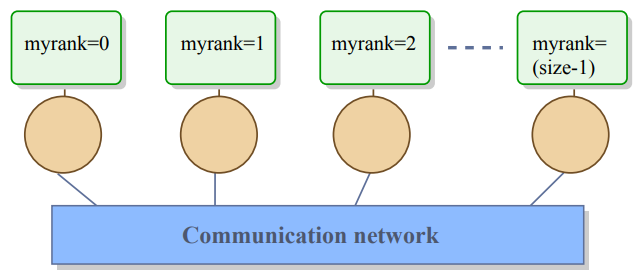
\includegraphics[height=0.4\textheight]{figures/MPI/Rank.png}
    \end{figure}
\end{frame}

\begin{frame}{Ngắt môi trường MPI}
    \begin{itemize}
        \item int MPI\_Finalize(): Ngắt kết nối môi trường MPI
        \item int MPI\_Abort(MPI\_Comm comm, int errorcode): Nếu một tiến trình bắt được một lỗi và không xử lý được
    \end{itemize}
\end{frame}

\begin{frame}[fragile]{Chương trình MPI Hello World}
    \begin{verbatim}
#include<stdio.h>
#include<mpi.h>
int main(int argc, char** argv) {
    int size, rank;
    MPI_Init(&argc, &argv);
    MPI_Comm_size(MPI_COMM_WORLD, &size);
    MPI_Comm_rank(MPI_COMM_WORLD, &rank);
    printf("From process %d out of %d processes", rank, size);
    MPI_Finalize();
    return 0;
}
    \end{verbatim}
\end{frame}

\begin{frame}{Truyền thông}
    \begin{itemize}
        \item Giao tiếp truyền thông điệp có thể giữa hai tiến trình hoặc giữa một nhóm các tiến trình
        \item Truyền thông thường là truyền mảng dữ liệu tổ chức theo kiểu dữ liệu MPI:
        \begin{itemize}
            \item Kiểu dữ liệu được định nghĩa là ánh xạ tớ kiểu dữ liệu của ngôn ngữ lập trình sử dụng MPI.
            \item Kiểu dữ liệu người do người dùng định nghĩa, các cấu trúc hoặc các kiểu dữ liệu khác
            \item Kiểu dứ liệu do người dùng định nghĩa sẽ được MPI tối ưu
        \end{itemize}
    \end{itemize}
\end{frame}

\begin{frame}{Các kiểu dữ liệu nguyên thủy của MPI}
    \begin{table}[H]
        \centering
        \begin{tabular}{ll}
            \hline
            Kiểu dữ liệu của MPI & Kiểu dữ liệu của C \\
            \hline
            MPI\_CHAR & signed char \\
            MPI\_SHORT & signed short int \\
            MPI\_INT & signed int \\
            MPI\_LONG & signed long int \\
            MPI\_UNSIGNED\_CHAR & unsigned char \\
            MPI\_UNSIGNED\_SHORT & unsigned short int \\
            MPI\_UNSIGNED & unsigned int \\
            MPI\_UNSIGNED\_LONG & unsigned long int \\
            MPI\_FLOAT & float \\
            MPI\_DOUBLE & double \\
            MPI\_LONG\_DOUBLE & long double \\
            MPI\_BYTE & 8 bits \\
            MPI\_PACKED & dãy bytes được đóng gói \\
            \hline
        \end{tabular}
    \end{table}
\end{frame}

\begin{frame}{Thông điệp}
    Một thông điệp bao gồm các trường thông tin:
    \begin{itemize}
        \item Địa chỉ người gửi
        \item Nơi lưu trữ thông điệp
        \item Kiểu dữ liệu thông điệp
        \item Kích thước thông điệp
        \item Thẻ thông điệp
        \item Địa chỉ người nhận 
        \item Nơi lưu trữ nhận thông điệp
        \item Kiểu dữ liệu phù hợp nơi nhận 
        \item Thẻ thông điệp khớp với bên gửi
    \end{itemize}
\end{frame}

\begin{frame}{Truyền thông điệp điểm - điểm}
    \begin{itemize}
        \item Giao tiếp blocking: Chờ đến khi truyền thông điệp hoàn thành
        \item Giao tiếp non-blocking: Trả về không cần đợi khi truyền thông điệp hoàn thành
        \item Các hình thức gửi:
        \begin{itemize}
            \item Đồng bộ: thông điệp chỉ được gửi khi biết chắc chắn có người đã sẵn sàng đợi nhận ở phía bên kia (fax).
            \item Bộ đệm: tin nhắn được gửi đi nếu người bên kia đang đợi hoặc nếu không sẽ được lưu vào một bộ đệm tạm thời cho đến khi lấy thông điệp khỏi bộ đệm.
            \item Kiểu sẵn sàng: giống như đồng bộ nhưng không có xác nhận từ bên nhận.
        \end{itemize}
    \end{itemize}
\end{frame}

\begin{frame}{Truyền thông điệp có blocking của MPI}
    \begin{itemize}
        \item int MPI\_Send(void *buf, int count, MPI\_Datatype datatype,
                            int dest, int tag, MPI\_Comm comm);
        \begin{itemize}
            \item buf là địa chỉ bắt đầu chứa thông điệp cần được truyền
            \item count là số phần tử của thông điệp
            \item datatype là kiểu dữ liệu của thông điệp
            \item dest là rank của tiến trình nhận thông điệp
            \item tag là một số định danh của thông điệp, thống nhất giữa bên gửi và bên nhận
            \item comm là bộ giao tiếp
        \end{itemize}
        \item Ví dụ: MPI\_Send(A, ns, MPI\_INT, 1, 0, MPI\_COMM\_WORLD): 
        Truyền ns phần tử kiểu int từ địa chỉ A sang tiến trình 1 với tag là 0.
    \end{itemize}
\end{frame}

\begin{frame}{Truyền thông điệp có blocking của MPI}
    \begin{itemize}
        \item MPI\_Ssend: Gửi đồng Bộ
        \begin{itemize}
            \item Người gửi thông báo người nhận, người nhận xác nhận sẵn sàng và người gửi gửi thông điệp.
        \end{itemize}
        \item MPI\_Bsend: Gửi bộ đệm
        \begin{itemize}
            \item Người gửi đưa dữ liệu và một bộ đệm và trả về ngay lập tức
        \end{itemize}
        \item MPI\_Rsend: Gửi sẵn sàng
        \begin{itemize}
            \item Người nhận được thông báo và dữ liệu được gửi ngay
        \end{itemize}
    \end{itemize}
\end{frame}

\begin{frame}{Một số lưu ý khi gửi thông điệp blocking}
    \begin{itemize}
        \item Đối với dữ liệu nhỏ, có thể dùng bộ đệm, đồng bộ phù hợp với dữ liệu lớn hơn
        \item MPI\_Ssend có thể gây ra deadlock
    \end{itemize}
\end{frame}

\begin{frame}{Hiệu năng của truyền thông điệp blocking}
    \begin{itemize}
        \item Truyền đồng bộ  cho tốc độ truyền dữ liệu cao nhất, nhưng chi phí khở tạo lại rất cao (độ trễ) và nguy cơ xảy ra deadlock.
        \item Truyền bộ đệm cho độ trễ thấp nhất nhưng:
        \begin{itemize}
            \item Quản lý bộ đệm phức tạp
            \item Vấn đề về băng thông do chi phí sao chép
        \end{itemize}
        \item Gửi sẵn sàng có vẻ là tốt nhất nhưng cũng rất dễ gây khó khăn trong lập trình nên cũng tránh sử dụng
        \item Truyền theo tiêu chuẩn cần phải được tối ưu cẩn thận. Với thông điệp kích thước lớn gần như chắc chắn xảy ra deadlock
    \end{itemize}
    
\end{frame}

\begin{frame}{Nhận thông điệp có blocking của MPI}
    \begin{itemize}
        \item int MPI\_Recv(void *buf, int count, MPI\_Datatype datatype,
                            int source, int tag, MPI\_Comm comm,
                            MPI\_Status *status)
        \begin{itemize}
            \item buf là địa chỉ bắt đầu chứa thông điệp nhận được
            \item count là số phần tử của thông điệp
            \item datatype là kiểu dữ liệu của thông điệp
            \item source là rank của tiến trình gửi thông điệp
            \item tag là một số định danh của thông điệp, thống nhất giữa bên gửi và bên nhận
            \item comm là bộ giao tiếp
            \item status là địa chỉ biến nhận trạng thái
        \end{itemize}
        \item Ví dụ: MPI\_Recv(B, ns, MPI\_INT, 0, 1, MPI\_COMM\_WORLD, \&status);
    \end{itemize}
\end{frame}

\end{document}